\section{Preliminaries}
% focusing on discrete at least for now, would be nice to show the connection to the real world through the continuous case
% \subsection{The continuous setting}
% Let our \emph{workspace} be defined as a finite space $W \coloneqq \nngrid \subset \rsquared$.
% In our workspace we have $N$ robots $R \coloneqq \set{1, 2, \dots , N} \subset \mathbb{N}$. 
% The \emph{positions} of the robots are defined by the center of their discs $v_i = \colvec{x}{y} \in \rsquared, \forall i \in R$, and they all have a \emph{constant radius 1}.
% We use the \emph{Euclidean norm} $L_2 = \euclnorm{p - q} \coloneqq \sqrt{(p_x - q_x)^2 + (p_y - q_y)^2}$ for any points $p, q \in \rsquared$ to measure distance.   
% The shapes of the robots are thus defined by the points within unit radius of their centers: $\set{p \mid \euclnorm{p - v_i} \leq 1} \subset \rsquared, \quad \forall i \in R$.
%
% The trajectory of a robot 
%
% The robots are not allowed to collide, which requires that they are disjoint: $\set{\euclnorm{v_i - v_j} \geq 2 \quad \forall i, j \in R \mid i \neq j}$.
%


% which are defined by their centers $x_i \in \rsquared$, $\forall i \in R$, and their radii, fixed at 1. 
% The robots define 


\subsection{A discrete grid of robots}
Let our grid-based workspace be modeled as a graph $G \coloneqq (V, E)$. 
Let it be a rectangle $\nngrid, \quad n_1, n_2 \geq 2$. 
Label the vertices as $V = \set{1, 2, \dots , n_1} \times \set{1, 2, \dots , n_2}$, and denote their $x$ and $y$ -coordinates as $v_x$ and $v_y$ respectively for any vertex $v \in V$.
To measure distance, we use the \emph{Manhattan norm} $L_1 = \manhattan{v - w} \coloneqq (\abs{v_x - w_x} + \abs{v_y - w_y})$.
Using this, the edges can be defined as $E = \set{(v, w) \mid \manhattan{v - w} = 1 \mid v, w \in V}$.
In other words, nodes are only connected to their up to four immediate neighbors in the plane.

A \emph{configuration} is an injective mapping $\conf{} : V \rightarrow \set{1, 2, \dots, N, \bot}$. 
Injective implies no two vertices in $V$ can be occupied at once, while $\bot$ signifies an empty vertex, so there will always be exactly $(\nngrid - N)$ empty squares in the grid. 

The \emph{inverse} of a configuration $\iconf{}{r} = (x, y), r \in R$ is the \emph{position} of a robot. 
The robots move synchronously and in parallel, a maximum of 1 square per step:
a configuration can thus be \emph{transformed} into another configuration in a \emph{single step} if and only if:

\begin{align}
	& \set{\iconf{1}{r} = \iconf{2}{r} \lor (\iconf{1}{r}, \iconf{2}{r}) \in E, \quad \forall r \in R}\label{req:limited_movement}\\
	\land & \set{\nconf{1}{v} = \nconf{2}{w} \Rightarrow \nconf{2}{v} \neq \nconf{1}{w}, \quad \forall v, w \in V}\label{req:no_swaps}
\end{align}

In other words, \cref{req:limited_movement} implies a robot can stay in place or move to a neighboring square at every step, while \cref{req:no_swaps} forbids two robots from swapping places in a single transformation step (and they can never occupy the same vertex), equivalent to a collision in the real world.

Denote a single transformation step as $\conf{1} \rightarrow \conf{2}$.
A \emph{schedule} is a series of transformation steps $\conf{1} \rightarrow \conf{2} \rightarrow \cdots \rightarrow \conf{k}$. 
A configuration $\conf{s}$ can be transformed into a configuration $\conf{t}$ if there exists a schedule $\conf{s} \rightarrow \conf{s + 1} \rightarrow \cdots \rightarrow \conf{t - 1} \rightarrow \conf{t}$.


\begin{definition}\label{def:motion_planning_problem}
	Given a start configuration $\conf{s}$ and a target configuration $\conf{t}$ of a workspace, 
	the \emph{motion planning problem} is to find a \emph{schedule} that transforms $\conf{s}$ into $\conf{t}$.
\end{definition}

\begin{remark}\label{remark:reachability}
	For a $2 \times 2$ square and any $1 \times n$ rectangle, where $n \geq 2$, there exist pairs of configurations that are not reachable from each other via any schedule. See \cref{fig:reachability} for an example.
	For any other rectangular workspace there always exists such a schedule. 
\end{remark}

\begin{figure}[h]
	\centering
	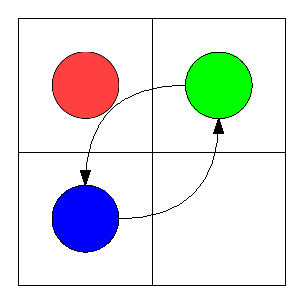
\includegraphics[width=4cm]{include/impossible_2x2.eps}
	\caption{A minimal example of an unsolvable motion planning problem: there exists no valid schedule which swaps the green and blue robots.}\label{fig:reachability}
\end{figure}

\begin{definition}\label{def:makespan}
	The number of single transformation steps in a schedule is called the \emph{makespan} of that schedule.
\end{definition}

\begin{definition}\label{def:optimality}
	A schedule $S_\text{opt}$ is \emph{optimal} by some metric $f : S \rightarrow \mathbb{R}$ iff $f(S) \geq f(S_\text{opt})$ for all valid schedules $S$.
\end{definition}


\begin{definition}
	Let the makespan of a schedule be such a metric: $M : S \rightarrow \text{\# steps in } S$.
	The \emph{minimum makespan motion planning problem} is to find an \emph{optimal} schedule to \cref{def:motion_planning_problem} with respect to the makespan $M$ of that schedule.
\end{definition}

\begin{remark}
	The \emph{minimum makespan} for any motion planning problem $\conf{s}$ and $\conf{t}$ has a lower bound of $\max(\set{\manhattan{\iconf{s}{r}, \iconf{t}{r}} \mid r \in R})$.
\end{remark}

\begin{definition}
	Let a schedule with makespan $M$ have the aforementioned lower bound as $L$.
	The $\emph{stretch factor}$ for that schedule is defined as $\frac{M}{L} \geq 1$.
\end{definition}

\subsection{Some notation}

\begin{definition}
	$O(g(x))$
\end{definition}






